\documentclass[UTF8]{ctexart}[a4paper,10pt]
\usepackage{hyperref}
\usepackage{amsmath}
\usepackage{amsfonts,amssymb} 
\usepackage{amsthm,thmtools}
\usepackage[hmargin=2.5cm,vmargin=2.5cm]{geometry}
\usepackage{tikz-cd,tikz}
\usepackage{graphicx,float}
\declaretheorem[numberwithin=section,style=definition,name=定义]{defn}
\declaretheorem[numberwithin=section,style=plain,name=定理]{thm}
\declaretheorem[numberwithin=section,style=plain,name=命题]{pro}
\declaretheorem[numberwithin=section,style=plain,name=例]{example}
\declaretheorem[numbered=no,style=definition,name=Remark]{remark}
\declaretheorem[numberwithin=section,style=plain,name=推论]{cor}
\declaretheorem[numberwithin=section,style=plain,name=引理]{lem}

\def\N{\mathbb{N}}
\def\Z{\mathbb{Z}}
\def\Q{\mathbb{Q}}
\def\R{\mathbb{R}}
\def\C{\mathbb{C}}
\def\S{\mathbb{S}}
\def\D{\mathbb{D}}
\def\H{\mathbb{H}}

\title{复变函数\uppercase\expandafter{\romannumeral2}期末作业:探讨从单位圆盘到多边形的全纯同胚}
\author{2010530 袁敏翔}

\begin{document}
    \maketitle
    
    \begin{abstract}
        Riemann映照定理优美地告诉我们,复平面上两个不为
        $\mathbb{C}$的单连通区域必然存在全纯同胚。
        但正如探险者知道了宝藏的存在却不知道
        其藏在何处,Riemann并没有告诉
        我们这样的全纯函数应该拥有什么样的形式。
        本文将探讨一类特殊的全纯同胚——
        从单位圆盘到多边形全纯同胚的具体形式,
        以此为其他情况下寻找全纯函数提供启发。

        声明:本篇论文基本参照了由E. M. Stein and R. Shakarchi. Complex analysis. Complex analysis, 2007.中的231页到245页的内容。
        在原书的基础上,加入了大量对文献逻辑结构和定理证明的思考。同时也有对文献中一些证明思路的补充和优化。
    \end{abstract}
    \tableofcontents
    
    \newpage
    \section{总体思路}
    应该怎样寻找我们所想要的全纯同胚?
    我们不妨先从我们已知的若干个全纯同胚来
    寻找一些灵感:
    \begin{example}
    我们将复平面的上半平面记为$\mathbb{H}$,
    将单位圆盘$V(0,1)$记为$\mathbb{D}$.
    由于两者都是复平面上不为$\mathbb{C}$的单连通区域,
    因此必然存在全纯同胚。事实上,我们已经给出了这样的全纯函数:
    $$
    F(z)=e^{i\lambda}\frac{z-\alpha}{z-\bar{\alpha}},\alpha \in \mathbb{H}
    $$
    
    我们不难发现这个事实:
    \begin{pro}
        考虑增广复平面,则$F: \mathbb{H}\rightarrow \mathbb{D}$可以延拓到两个区域的边界上。
        即$F$同时也是从增广实数轴到单位圆的连续双射。
    \end{pro}
    \begin{proof}
        首先将$F$看作$\overline{\mathbb{C}}$的函数。这个函数在$\overline{\mathbb{C}}$是解析双射的。我们只需要验证这样的延拓是良定的。
        
        如果$x\in \mathbb{R} $,那么
        $$
        |F(x)|=|\frac{x-\alpha}{x-\bar{\alpha}}|=|\frac{x-\alpha}{\overline{x-\alpha}}|=1
        $$.

        如果$|F(z)|=1$,那么
        $$
        |z-\alpha|=|z-\overline{\alpha}|
        $$
        从几何上看,很容易知道$z$在实轴上。同时如果$|z|=\infty$,等式也成立。

        因此,$F$同时也是从增广实数轴到单位圆的连续双射。
    \end{proof}
    \end{example}
    \begin{example}
    我们也探讨了$\mathbb{D}$到自身的全纯同胚。这样的同胚拥有的形式是:
        $$
        G(z)=e^{i\lambda}\frac{z-\alpha}{1-\overline{\alpha}z}, \quad \alpha \in \mathbb{D} 
        $$
    
        我们不难验证,这样的全纯同胚也满足1中延拓的性质:
        \begin{pro}
            考虑增广复平面,则$F: \D \rightarrow \mathbb{D}$可以延拓到两个区域的边界上。
            即$F$同时也是从单位圆到单位圆的连续双射。
        \end{pro}
        证明从略。 
    \end{example}
    \begin{example}
    考虑$S=\{z\in \C :0 < arg(z) < \pi/n \},0<n<2$.则这是一个单连通区域,且应该存在一个全纯同胚$f:S\rightarrow \H$。
      
      我们不假思索就能给出$f$的一个形式:
      $$
      f(z)=z^n
      $$
    
    我们不难验证,这样的全纯同胚也满足1中延拓的性质:
    \begin{pro}
        考虑增广复平面,则$f: S \rightarrow \mathbb{H}$可以延拓到两个区域的边界上。
    \end{pro}

    \end{example}

    上述三个例子实际上描述了一个事实:尽管全纯同胚只是两个区域之间的映射,但是我们可以把其延拓到两个区域的边界上,使得映射成为两个闭集间的连续双射。
    当然这里不谈解析,因为边界上的点很难谈论“解析”这件事。

    那么反过来,我们是否可以利用全纯函数的这样的性质,先诱导两个区域的边界间的双射,
    再根据边界的一些特征精确的描述该双射的具体形式,最后返回来证明其也是两个区域之间的解析双射?
    
    这实际上就是我们完成这项工作的思路.
    \section{边界行为}
    然而在我们信心满满开始寻找边界上的函数形式之前(如果我们想要找到全部的全纯同胚),我们必须首先证明,我们的函数能够延拓到边界上。事实上,有如下定理:
    \begin{thm}
        如果$F:\D \rightarrow P$是一个从单位圆盘映射到一个多边形的全纯同胚,
        那么$F$可以自然地被延拓为从$\overline{\D}$到$\overline{P}$的连续双射。
        并且$F$同时也给出了从$S$到$\mathfrak{p}$的连续双射,即$F(S)=\mathfrak{p}$。
        其中,$S=\{z:|z|=1\}$,$\mathfrak{p}$表示多边形。
    \end{thm}
    定理证明关键点在于:由于$F$延拓后的函数仍然是连续的,如果$z_0 \in S$,则必然有$\lim_{z \to z_0}F(z)$存在。因此我们的证明分为两个步骤:
    
    1.验证这个极限的存在。

    2.定义$F(z_0)=\lim_{z \to z_0} F(z)$,其中$z_0 \in S$.这样就保证了$F$的良定性。然后验证其是否满足双射和连续。

    \subsection{极限的存在性}
    \begin{lem}
        记$z_0$是$S$上的一个点,并记$D_r=\{z:|z-z_0|=r\}$。
        
        设$\rho(r)=sup_{z_r,z_r^{'}\in D_r\cap D }|F(z_r)-F(z_r^{'})|$,则存在一个数列$\{r_n\}_{n=1}^{\infty}$,使得:
        $$
        \lim_{n\to \infty}r_n=0     , \quad   \lim_{n\to \infty}\rho(r_n)=0
        $$
    \end{lem}
    下面的图给出了这个引理的情况。
    \begin{figure}[H]
        \centering
        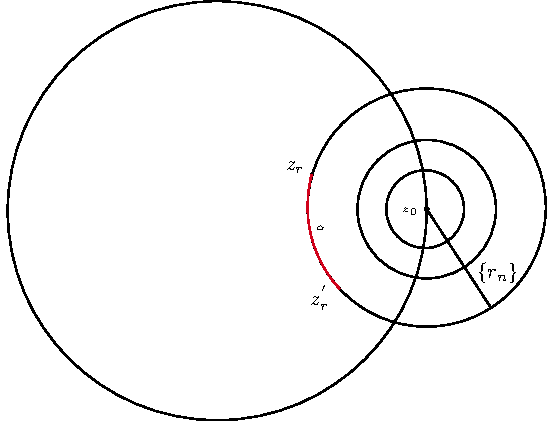
\includegraphics[scale=0.4]{引理1.pdf}
    \end{figure}
    从柯西审敛原理来看,如果$\lim_{z \to z_0} F(z)$存在,那么对于$\forall \epsilon>0$,总$\exists \delta>0$使得,
     $\forall z_1,z_2 \in \{z:|z-z_0|<\delta\}$,都有$|F(z_1)-F(z_2)|<\epsilon$。但上面的引理只告诉了我们,存在一个半径列,使得
     以这个列为半径的圆弧列上的每一个圆弧为定义域的$F(z)$的极差趋近于0.这是一个比柯西审敛原理弱很多的条件。但借助解析函数的良好性质,
     我们就能够证明极限的存在性。
    \begin{proof}
        使用反证法。如果不存在这样一个$\{r_n\}$,那么必然存在$R>0$和$c>0$,使得对于任何的$r:0<r<R$,都有$\rho(r)>0$。

        由于$\rho(r)\displaystyle=\sup_{z_r,z_r^{'}\in D_r\cap D }|F(z_r)-F(z_r^{'})|$,因此存在两个函数$z_r,z_r^{'},|z_r|=|z_r^{'}|=r$,使得:
        $$
        f(z_r)-f(z_r^{'})=\int_{\alpha} f^{'}(z)dz 
        $$
        
        其中$\alpha$表示连接$z_r,z_r^{'}$的一段弧。换元$z=z_0+re^{i\theta}$,并记还原后区间为$\theta_1(r)<\theta<\theta_2(r)$,那么
        $$
        \rho(r)\leq \int_{\theta_1(r)}^{\theta_2(r)}|f^{'}(z)|rd\theta
        $$
        
        使用柯西施瓦兹不等式:
        $$
        \rho(r)\leq \left(\int_{\theta_1(r)}^{\theta_2(r)}|f^{'}(z)|^2rd\theta)^{1/2}\right)\left(\int_{\theta_1(r)}^{\theta_2(r)}rd\theta\right)^{1/2}
        $$
        
        则有:
        $$
        \frac{\rho(r)^2}{r}\leq 2\pi \int_{\theta_1(r)}^{\theta_2(r)}|f^{'}(z)|^2rd\theta
        $$

        再次积分:
        $$
        c^2 \int_0^R \frac{dr}{r} \leq 2\pi \int_0^R \int_{\theta_1(r)}^{\theta_2(r)}|f^{'}(z)|^2rd \theta dr \leq 2\pi \iint_{\D}|f^{'}(z)|^2dxdy
        $$
        (这里用到了一个面积公式)
        然而不等式左边是不收敛的!因此这产生了一个矛盾。从而原命题是成立的。
    \end{proof}
       现在我们利用引理来证明极限的存在。
    \begin{thm}
       记$z_0$是单位圆上的一个点。那么$\lim_{z \to z_0}F(z)$存在。其中$z$是$\D$中的点,且趋近于$z_0$。
    \end{thm}
    \begin{proof}
        如果这个极限不存在,那么必然存在两个点列$\{z_n\},\{z_n^{'}\}$,它们同时趋近于$z_0$,
        但$\{F(z_n)\},\{F(z_n^{'})\}$却趋近于不同的$\omega,\omega^{'}$.

        由于$F$是一个解析同构,因此$\omega,\omega^{'}$均在$\mathfrak{p}$上。因此我们可以选择两个不相交的圆盘$D,D^{'}$,分别以$\omega,\omega^{'}$为圆心。

        取足够大的$n$,使得$\{F(z_n)\}\in D ,\{F(z_n^{'})\} \in D^{'}$

        因此,存在两条连续的曲线$\Lambda \in D \cap P ,\Lambda^{'}\in D^{'} \cap P$,分别穿过$\{F(z_n)\},\{F(z_n^{'})\}$。并且由于收敛性,这两条曲线的末尾点分别为$\omega,\omega^{'}$

        考虑$\lambda=F^{-1}(\Lambda),\lambda^{'}=F^{-1}(\Lambda^{'})$,则$\lambda,\lambda^{'}$是$\D$靠近$z_0$的两条曲线。

        通过引理2.1,我们知道这两条曲线对应的像之间的距离$d=inf_{\omega_1\in \Lambda,\omega_2\in \Lambda^{'}}|\omega_1-\omega_2|$为零。然而,由于$\Lambda \in D \cap P ,\Lambda^{'}\in D^{'} \cap P$
        在两个不相交的圆盘内,他们之间的距离又不可能为零。因此这产生了一个矛盾!

        故极限是存在的。
    \end{proof}
    \begin{figure}[H]
        \centering
        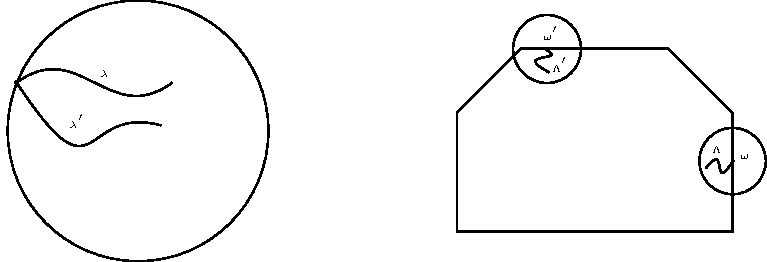
\includegraphics[scale=0.8]{定理2.2.pdf}
    \end{figure}
    \subsection{延拓后的函数是连续的双射}
    一旦极限存在,我们就可以定义$F(z)$在单位圆盘边界上的值。同理,对于$F$的反函数也可以如此操作。接下来我们只需要验证:

    1.$F$延拓后是连续的。

    2.$F$和$G$延拓后仍然互为反函数。

    \begin{proof}
        \quad

        对于第一条,我们只需要考虑圆环上两点靠近时,是否对应函数值也足够近。
        
        事实上,若$z \in S$且$|z-z_0|<\delta$,那么选择$\omega$使得$|F(\omega)-F(z)|<\epsilon$,且$|\omega-z_0|<\delta$.则:
        $$
        |F(z)-F(z_0)|\leq|F(z)-F(\omega)|+|F(\omega)-F(z_0)|<2\epsilon
        $$
        
        因此延拓后$F$连续。

        对于第二条,同理我们可以得到延拓后的$G$。则对于任何$z \in \partial D$,$G(F(z_k))=z_k$。在等式两边取极限$z_k \to z$,则有$G(F(z))=z$。同理$F(G(\omega))=\omega,\forall \omega \in \partial P$。
        
        因此延拓后两个函数仍互为相反数。
    \end{proof}
    \section{给出形式}
    \subsection{从把实数轴弯折开始}
    由于单位圆盘的边界并不是那么简单,而上半平面$\H$的边界却足够的简单清楚——仅仅只是实数轴。
    因此我们不妨把问题转化为从上半平面到多边形的映射——只需要最后复合上我们熟知的同胚就可以了。
    
    我们首先需要思考,什么样的映射可以把实数轴进行一个弯折?

    幸运的人总能在最美好的时间找到这个映射——例1.3。
    \begin{example}
        $$
        F(z)=z^{\alpha}
        $$
        可以把负半轴映射到$\{z:z=re^{i\alpha \pi}\}$。正好在原点处将负半轴折到了另一条轴上。  
    \end{example}
   

    但我们显然希望我们的函数能够把实轴弯折多次。让我们来考察上述函数在弯折处的特点:

    $F(z)=z^\alpha$在零点处取到了零值,接着从原来的方向扭转了$\alpha \pi$的角度,继续向另外一个方向延申。
    如果我们考虑积分的角度,我们可以看到,在零点后,$F^{'}(z)$的方向发生了变化。而对于一个一般的点,如果我们想要多边形在这个点发生偏折,也可以考虑这个点处,导函数的方向发生了突变。

    什么样的函数可能会呢?我们发现,如果对于函数$F^{'}(z)$,在零处,根式下的值发生了正负的变化,从而可以提出来一个虚数单位$i$。
    这多出来的虚数单位就可以扭转导函数的的方向。事实上,我们可以把这个思想放在其它一些例子验证:
    \begin{example}
    $$
    f(z)=\int_0^z\frac{d\omega}{(1-\omega^2)^{1/2}}
    $$
    将实数轴映射到下图的红线上:
   
    \begin{figure}[H]
        \centering
        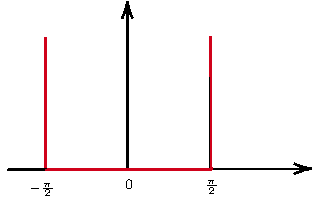
\includegraphics[scale=0.8]{例3.2.pdf}
    \end{figure}
    首先说明,式子中的根号对应的解析分支是让正数被开方为正数的解析分支。

    当$-1\leq x\leq1$的时候,根号下的数是正数,因此开方后,我们得到的也是正数。由于$f(0)=0$,因此$f(-1\leq x\leq 1)=-\frac{\pi}{2}\leq f\leq \frac{\pi}{2}$。
    当$x>1$,我们有:
    $$
    \frac{1}{(1-x^2)^{1/2}}=\frac{i}{(x^2-1)^{1/2}}
    $$
    等式右边的函数值正好只增长$f(z)$的虚部。根据积分,当$x>1$后,图中红色的线向上延伸。

    当$x<-1$的时候,情况是相似的。
    \end{example}
    \begin{pro}
    更一般的,如果函数$f(z)=\dfrac{g(z)}{(z-A_k)^{\alpha}},0<\alpha<2$,
    其中$g(x)$在$A_k$附近不变号,$A_k\in \R$。那么在$A_k$附近有:
   $$
    f(x)=\frac{g(x)}{(x-A_k)^\alpha},x>A_k
    $$
    $$
    f(x)=\frac{g(x)}{(A_k-x)^\alpha}(e^{i\pi})^\alpha,x<A_k
   $$
    因此,如果记$F(z)=\displaystyle\int_{A_0}^{z}f(\omega)d\omega$,$F(A_k)=a_k$,
    其中$A_0<A_k$,那么在$a_k$处,$F(z)$的像会发生一个弯折,弯折角为$\alpha \pi$.
    \end{pro}
    \subsection{Schwarz-Christoffel积分}
    研究了如何把实数轴给弯折后,我们就可以开始构造我们的映射了。经过上面的讨论,这应该是比较容易的:
    \begin{defn}
        给定实数$A_1<A_2<A_3<\cdots<A_n$和实数$\beta_1,\beta_2,\beta_3,\cdots,\beta_n$.其中$\beta_k<1,k=1,2,\cdots,n$
        且$\displaystyle \sum_{k=1}^n\beta_k>1$。称如下的积分是上述$2n$个实数对应的Schwarz-Christoffel积分:
        $$
        S(z)=\int_0^z \frac{d\zeta}{(\zeta-A_1)^{\beta_1}\cdots(\zeta-A_n)^{\beta_n}}
        $$
        其中,$(z-A_k)^{\beta_k}$是定义在除$U_k=\{A_k+iy:y\leq 0\}$外的复平面上的函数,
        其值域的解析分支,取使得$x>A_k$时所得到的函数值为正的解析分支。
    \end{defn}
    关于定义,我们还需要做一些说明:

    1.对于积分的奇点$A_1,\cdots,A_n$,由于$\beta_k<1$,因此在此处的广义积分收敛,从而可以$S(z)$的定义域包括$A_1,\cdots,A_n$。

    2.由于
    $$
    \left|\prod_{k=1}^n (\zeta-A_k)^{-\beta_k}\right|\leq c|\zeta|^{-\sum\beta_k} 
    $$
    在$\zeta$足够大的时候成立,因此$S(z)$在$\infty$处拥有定义。从而$S(z)$的定义域
    为$\overline{\D}\setminus\displaystyle\cup_{k=1}^n U_k$.同时,这一定义域是单连通的。

    3.$S(z)$在其定义域上解析。$S^{'}(\zeta)=\dfrac{1}{(\zeta-A_1)^{\beta_1}\cdots(\zeta-A_n)^{\beta_n}}$

    4.为方便起见,我们记$a_k=S(A_k),a_\infty=S(\infty)$。
    
    结合3.1节的讨论,我们有如下命题:
    \begin{pro}
        假设$S(z)$已经由上述方式定义,则:

        $(i)$如果$\sum_{k=1}^n \beta_k=2$,则$S(z)$将实数轴映射到由$a_1,a_2,\cdots,a_n$依次按顺序所连成的$n$多边形$\mathfrak{p}$。
        另外$a_\infty$位于$[a_n,a_1]$连线,且在$a_k$处形成的内夹角为$(1-\beta_k)\pi=\alpha_k \pi$。

        $(ii)$如果$1<\sum_{k=1}^n \beta_k<2$,则$S(z)$将实数轴映射到由$a_1,a_2,\cdots,a_n,a_\infty$依次按顺序所连成的$n+1$多边形$\mathfrak{p}$。
        且在$a_k$形成的内夹角依然为$(1-\beta_k)\pi=\alpha_k \pi$,在$a_\infty$处形成的内夹角为$(1-\sum_{k=1}^n \beta_k)\pi$.
    \end{pro}
    凭借对实数轴弯折的理解,命题的证明是显然的。因此我们略去证明。
    \subsection{构造积分的思路}
    凭借3.1节的讨论,实际上构造出$S(z)$的思路是不困难的。
    
    根据命题3.1,如果我们先预设好,
    在$A_1<A_2<\cdots<A_n$处实数将发生弯折角度$(1-\beta_k)\pi$的角度(实数轴会往上弯),那么对于$x=A_k$的附近,我们可以令:
    \begin{equation*}
        F(z)=\int_0^{z}\frac{p_k(z)}{(z-A_k)^{\beta_k}}dz
    \end{equation*}
    $p_k(z)$在$x=A_k$处附近不变号
    
    如何确立$p_k(z)$呢?不难发现,由于$A_1,A_2,\cdots,A_n$是孤立的,因此我们只需要让函数满足上述施瓦兹——克里斯托夫积分就可以了。
    这样构造出来的积分,我们还需要考虑:

    1.是否会弯折几周?——反映到$\sum \beta_k\leq 2$的条件。

    2.无穷远处怎么理解?——反映到是否能真正弯曲正好一周。不能的话,还会存在一个夹角。
    \section{最后的验证}
    我们目前已经做完了2/3的工作。现在我们将进入最后一部分:验证我们找到的函数$S(z)$是从$\H$到$P$的全纯同胚。

    我们不妨再理清一下逻辑:首先我们证明了,任何一个全纯同胚都可以自然的延拓为对应区域取闭集后的连续双射。
    因此我们可以从寻找合适的,可以将边界双射到边界的函数开始。由于所有的全纯同胚都是可以延拓的,因而我们不会遗漏。
    
    找到函数后,我们要做的,就是验证其是否真的可以成为全纯同胚。为方便起见,我们不再考虑无穷点的情况。即无穷点不对应为多边形的顶点。

    \begin{thm}
        记$P$是一个多边形的内部。$F:\H \to P$是两个区域之间的全纯同胚。将$F(z)$延拓后,记多边形的$n$个顶点$a_1,\cdots,a_n$
        所对应的实数轴上的点分别为$A_1,\cdots,A_n$。每个顶点的内角为$\alpha_1\pi,\cdots,\alpha_n\pi$,记$\beta_k=1-\alpha_k$,
        那么$F(z)=c_1S(z)+c_2$,其中S(z)是由上述$A_k$和$\beta_k$2n个点所给出的Schwarz-Christoffel积分,$c_1$和$c_2$是两个常数,
        由$P$自身决定。
    \end{thm}
    \begin{proof}
        我们首先考虑上半平面中位于$[A_{k-1},A_k]$和$[A_{k},A_{k+1}]$之上的部分。注意到$F$把这两个区间分别映射到两个相交于$a_k=F(A_k)$的线段,并且夹角为$\alpha_k\pi$.
        
        定义:
        $$
        h_k(z)=(F(z)-a_k)^{1/\alpha_k}
        $$
        其中,$z$的取值范围,是一个由$Re(z)=A_{k-1}$和$Re(z)=A_{k+1}$为边界(但不包含这两条边界线),只包括实轴上半部分的区域。开根号的解析分支是选定的。

        $h_k$也可以延拓到$(A_{k-1},A_{k+1})$区间上。由于指数$1/\alpha_k$的存在,$h_k(z)$把此处的折线拉直。从而:
        $$
        h_k([A_{k-1},A_{k+1}])=L_k
        $$
        $L_k$是一条(而非有弯折的)位于复平面上的线段。并且这条线段穿过$0$($h_k(A_k)=0$).
        
        从而我们只需要为$h_k(z)$乘一个旋转的因子,就可以应用Schwarz对称定理。对称后再利用相反的旋转因子,就可以将$h_k(z)$的值域延拓到$L_k$另一边。
        我们记$H_k(z)$为延拓后的函数,$\Omega_k$为延拓后的定义域$\Omega_k=A_{k-1}<Re(z)<A_{k+1}$。根据Schwarz对称定理,这个函数是解析的。
        
        断言:$H'_k(z)\neq 0$.

        事实上,如果$Im(z)>0$,那么:
        $$
        \frac{F'(z)}{F(z)-F(A_k)}=\alpha_k\frac{H^{'}_k(z)}{H_k(z)}
        $$
        由于$F$是解析双射,则$F'(z)\neq 0$。故$H'_k(z)\neq0$.

        根据对称定理,$H'_k(z)$在$\{z:Im(z)<0\}$的位置也不为$0$。

        当$z\in \R$,取一个足够小的圆,以$z$为圆心。由于单纯把$h_k$延拓到实轴上时,所得到的函数仍然是连续双射。而根据对称定理,这个圆下方的,$H_k(z)$的函数值也不能等于实轴上$H_k(z)$的函数值。
        因此在小圆中,$H_k(z)$是一个单射。从而,$H'_k(z)\neq 0$.

        因为$H'_k(z)\neq0$,
        而$F'=\alpha_kh_k^{-\beta_k}h'_k$,$F''=-\beta_k\alpha_kh_k^{-\beta_k-1}(h'_k)^2+\alpha_kh_k^{-\beta_k}h''_k$,
        从而我们可以进行把$F',F''$自然的延拓到$\Omega_k\setminus{A_k}$上(即我们直接把$h_k$替换为$H_k$).延拓后,记$F$为$\mathcal{F}_k$,从而有:
        $$
        \frac{\mathcal{F}_k''(z)}{\mathcal{F}'_k(z)}=-\frac{\beta_k}{z-A_k}+E_k(z)
        $$
        其中,$E_k$是$\Omega_k$上的解析函数。

        同理,对于$k=1$和$k=n$,我们也有类似的结论。只是$\Omega_1=-\infty<Re(z)<A_{k+1}$,$\Omega_n=A_{n}<Re(z)<\infty$.

        由于$F$把实轴映射到多边形的边,因此,$F([-\infty,A_1)\cup(A_n,\infty])=(a_n,a_1)$。
        因此,我们可以在这样的情况下对$F$直接使用Schwazr对称定理。延拓后记为$\mathcal{F_\infty}$(实际上,因为无穷远点没有弯折)

        注意到,同一个位于实轴上方的点,其延拓后的结果应该不变(解析函数唯一性定理)。即
        $$
        \mathcal{F}_k(z)=\mathcal{F}_{k+1}(z),\forall z,Re(z) \in (A_k,A_{k+1})
        $$
        同时,每个$\mathcal{F}_k$的边界线$\{z:z=A_{k-1}+iy,y\in \R,y\neq 0\} \{z:z=A_{k+1}+iy,y\in \R \neq 0\}$正好可以由相邻区域块的内部来补充,
        因此我们可以合并$\mathcal{F}_k$与$\mathcal{F_\infty}$
        ,记为一个函数$\mathcal{F}$。$\mathcal{F}$在$\H$的取值正好是$F$.且$\mathcal{F}$的定义域只挖去了$A_k$。
        
        而$F(\H)=P$,故延拓后,$\mathcal{F}$在无穷远处也是有界的,因而是一个可去奇点。从而$\mathcal{F}$的Luarant级数在无穷远处没有正数项。

        因而,$\mathcal{F}''/\mathcal{F}'$在无穷远处是解析的,并且收敛于0。

        接下来我们考察:
        $$
        G(z)=\frac{\mathcal{F}''(z)}{\mathcal{F}'(z)}+\sum_{k=1}^{n}\frac{\beta_k}{z-A_k}
        $$
        虽然在$\{z:z=A_1,A_2,\cdots,A_k\}$处,两个函数都是不解析的。但是由于之前的分析,他们的和在这上面却是解析的。
        并且根据$\mathcal{F}''/\mathcal{F}'$在无穷远处收敛于0,得到$G(z)$是整个复平面上的有界整函数。故$G(z)=0$.

        故我们得到了一个关于$F(z)$的微分方程。

        可以解得:$F'(z)=c(z-A_1)^{-\beta_1}\cdots (z-A_n)^{-\beta_n}$

        再进行一次积分,我们便得到了我们梦寐以求的$F$。
        \end{proof}
   

    定理的证明重在Schwarz对称定理的应用。通过延拓,并且构造了合适的整函数,正好给出了我们想要的形式。
    证明中把折线“掰直”的想法也是颇为精妙的,值得我们反思和思考。
    \cite{2007Complex}

    
    至此,我们便找到了想要的全纯同胚。
    \bibliographystyle{plain}
    \bibliography{math}
\end{document}